%%
%% This is file `sample-sigconf.tex',
%% generated with the docstrip utility.
%%
%% The original source files were:
%%
%% samples.dtx  (with options: `sigconf')
%% 
%% IMPORTANT NOTICE:
%% 
%% For the copyright see the source file.
%% 
%% Any modified versions of this file must be renamed
%% with new filenames distinct from sample-sigconf.tex.
%% 
%% For distribution of the original source see the terms
%% for copying and modification in the file samples.dtx.
%% 
%% This generated file may be distributed as long as the
%% original source files, as listed above, are part of the
%% same distribution. (The sources need not necessarily be
%% in the same archive or directory.)
%%
%% The first command in your LaTeX source must be the \documentclass command.
\documentclass[sigconf]{acmart}

% TODO remove XD
\usepackage{xcolor}
\newcommand{\secfunc}[1]{{\color{magenta}#1}}
\newcommand{\mention}[1]{{\color{cyan}#1}}
\newcommand{\plan}[1]{{\color{purple}#1}}
\newcommand{\bp}[1]{{\color{violet}#1}}
\newcommand{\draft}[1]{{\color{blue}#1}}
\newcommand{\review}[1]{{\color{black}#1}}
\newcommand{\todo}[1]{{\color{orange}#1}}
%%
%% \BibTeX command to typeset BibTeX logo in the docs
\AtBeginDocument{%
  \providecommand\BibTeX{{%
    \normalfont B\kern-0.5em{\scshape i\kern-0.25em b}\kern-0.8em\TeX}}}

%% Rights management information.  This information is sent to you
%% when you complete the rights form.  These commands have SAMPLE
%% values in them; it is your responsibility as an author to replace
%% the commands and values with those provided to you when you
%% complete the rights form.
\setcopyright{acmcopyright}
\copyrightyear{2018}
\acmYear{2018}
\acmDOI{10.1145/1122445.1122456}

%% These commands are for a PROCEEDINGS abstract or paper.
\acmConference[Woodstock '18]{Woodstock '18: ACM Symposium on Neural
  Gaze Detection}{June 03--05, 2018}{Woodstock, NY}
\acmBooktitle{Woodstock '18: ACM Symposium on Neural Gaze Detection,
  June 03--05, 2018, Woodstock, NY}
\acmPrice{15.00}
\acmISBN{978-1-4503-9999-9/18/06}


%%
%% Submission ID.
%% Use this when submitting an article to a sponsored event. You'll
%% receive a unique submission ID from the organizers
%% of the event, and this ID should be used as the parameter to this command.
%%\acmSubmissionID{123-A56-BU3}

%%
%% The majority of ACM publications use numbered citations and
%% references.  The command \citestyle{authoryear} switches to the
%% "author year" style.
%%
%% If you are preparing content for an event
%% sponsored by ACM SIGGRAPH, you must use the "author year" style of
%% citations and references.
%% Uncommenting
%% the next command will enable that style.
%%\citestyle{acmauthoryear}

%%
%% end of the preamble, start of the body of the document source.
\begin{document}

%%
%% The "title" command has an optional parameter,
%% allowing the author to define a "short title" to be used in page headers.
\title{Analyzing Build Logs Using Programming by Example}

\author{Carolin Brandt}

%%
%% By default, the full list of authors will be used in the page
%% headers. Often, this list is too long, and will overlap
%% other information printed in the page headers. This command allows
%% the author to define a more concise list
%% of authors' names for this purpose.
\renewcommand{\shortauthors}{Brandt, et al.}

%%
%% The abstract is a short summary of the work to be presented in the
%% article.
\begin{abstract}
  ...
\end{abstract}

%%
%% The code below is generated by the tool at http://dl.acm.org/ccs.cfm.
%% Please copy and paste the code instead of the example below.
%%
%\begin{CCSXML}
%<ccs2012>
% <concept>
%  <concept_id>10010520.10010553.10010562</concept_id>
%  <concept_desc>Computer systems organization~Embedded systems</concept_desc>
%  <concept_significance>500</concept_significance>
% </concept>
% <concept>
%  <concept_id>10010520.10010575.10010755</concept_id>
%  <concept_desc>Computer systems organization~Redundancy</concept_desc>
%  <concept_significance>300</concept_significance>
% </concept>
% <concept>
%  <concept_id>10010520.10010553.10010554</concept_id>
%  <concept_desc>Computer systems organization~Robotics</concept_desc>
%  <concept_significance>100</concept_significance>
% </concept>
% <concept>
%  <concept_id>10003033.10003083.10003095</concept_id>
%  <concept_desc>Networks~Network reliability</concept_desc>
%  <concept_significance>100</concept_significance>
% </concept>
%</ccs2012>
%\end{CCSXML}
%
%\ccsdesc[500]{Computer systems organization~Embedded systems}
%\ccsdesc[300]{Computer systems organization~Redundancy}
%\ccsdesc{Computer systems organization~Robotics}
%\ccsdesc[100]{Networks~Network reliability}

%%
%% Keywords. The author(s) should pick words that accurately describe
%% the work being presented. Separate the keywords with commas.
\keywords{ci, buildlogs, programming by example}

%%
%% This command processes the author and affiliation and title
%% information and builds the first part of the formatted document.
\maketitle


\secfunc{section function - \textbackslash secfunc} \\
\mention{things to mention / reference - \textbackslash mention} \\
\plan{what to write here - \textbackslash plan} \\
\bp{actual bullet points - \textbackslash bp} \\
\draft{final text drafty - \textbackslash draft} \\
\review{final text review ready - \textbackslash review} \\
\todo{ToDo - \textbackslash todo} \\

\section{Introduction}
\secfunc{why? what? research questions? purpose? hypothesis? wide $\rightarrow$ narrow

problem, done in literature, why not enough? our approach
}

\review{Fixing a broken continuous integration (CI) build has a high priority for developers~\cite{vassallo2018un-break}, therefore decreasing the time until the success build state is restored improves the overall productivity of developers.

\plan{why are logs so difficult: mention heterogeneous, semi-structured (paper reference for that?), big data (reference paper about log sizes), in distributed systems probably distributed (really also for build log?)

to combat that users write tools to <extract / retrieve superbegriff> information from build logs.

one possibility IR: classify specific part of program as similar to others (list IR technique) to see whether it is correlated to a failure. but not as good: not a real summarization technique, more what is similar to the last few times it failed.

way to extract fine grained information: regular expressions which have to be written manually

\todo{maybe other paragraph. here only half fitting?}
}

During this assignment an engineer spends a lot of their time \todo{or: find percentage to cite} reading very long and verbose build logs, trying to retrieve the relevant information from between many uninteresting other lines. \todo{add anecdotal evidence, watchdog paper?}

A way to support them would be to extract the desired information and present it in a structured way.
One approach to realize such functionality are tools that employ handcrafted regular expressions to find the desired text parts within the build log.
However, creating these regular expressions is tedious, mentally complicated and usually error-prone task. Especially when they have to be maintained for long \textemdash \ reunderstanding old regular expressions is known to be a dreading task for developers.
Our goal is to evaluate an alternative way of taking this burden of programmers.
By simply giving examples of the desired extractions they should be able to define extraction programs.

We implement \todo{<toolname, ALBE?, Analyzing Logs By Example>}, a prototype for defining text extractions from build logs through examples.
After collecting a diverse set of build logs from Travis CI we design a meta-model of the contained information.
We evaluate ALBE on logs from selected GitHub repositories on the accuracy of extraction for a varying number and selection of in-output-examples.
Furthermore we compare the tool to classical information retrieval and plain keyword search.
Our evaluation of ALBE shows that it is able to define extractions for various desired informations, that it shortens development time in comparison to manual regular expression construction and ...
}

\todo{Research Questions!}

\bp{ RQ1: how many and which kind of samples does pbe need to be competitive with existing methods? }

\bp{ can pbe extraction replace or even exceed existing methods for our use case? }

\bp{ What are the limitations of extractions? (only interesting when specified with PROSE library..)}

\bp{ Adjustements / Improvements to PROSE for extracting specifically from build logs }

\section{Related Work}

\todo{More glue \& sentences that give an overview over the next paragraph}
	
\subsection{Bulidlogs Analysis Tools}

\review{
Vassallo et al.~\cite{vassallo2018un-break} tried to shorten the time it takes developers to understand build logs. They summarized relevant information in Maven build logs and augmented them with links to related stack overflow posts. They observed that highlighting the locality and context of an issue is helpful to programmers. We strive to enable a similar summarization by text extraction while also covering a wider array of programming languages.

Amar et al.~\cite{amar2019mining} reduced the lines of a log to be inspected by the engineer through removing lines that appear both in passing and failing build logs. They further employed information retrieval techniques to identify the lines most likely hinting at the cause of the error. In contrast to that, our tool ALBE extracts specific parts of the build logs. As this is mostly dependent on the implicit reoccurring structure within the logs we operate on the full log output.
}

\subsection{Continuous Integration}

\review{
Various researchers have analyzed industrial and open source logs for failure reasons and their impact on development. Seo et al.~\cite{seo2014programmers} found that few error types such as dependency mismatches are the most prominent cause of build failures at Google. In addition most failures are resolved within two builds. Vassallo et al.~\cite{vassallo2017a-tale} compared open source projects in Java to industrial ones. They determined that testing failures outweigh compilation errors. Open source builds fail most often because of unit tests, whereas release preparations is the primary cause in industrial projects. Beller et al.~\cite{beller2017oops} showed that testing is central to continuous integration when evaluating Travis CI logs for Java and ruby builds. They observed very different kinds, failure rates and numbers of test between programming languages and explained that the low failure rates hint at code being tested before it is sent to the CI server.

All these researchers described building parsers in order to evaluate the studied build logs. Our work could support their research by easing the parser development and enable them to cover more languages and build tools easier.
}


\subsection{Information Extraction and Retrieval}

\review{Getting the general topic or conceptual information of a text is a common task in information retrieval from semi-structured text sources. Usually this is done by preprocessing the documents, transforming them to a term-by-document matrix. On the matrix we apply a similarity comparison like for example vector space models to calculate the similarity of the different documents to each other~\cite{panichella2016parameterizing}. For our use case, this could be applied by slicing the build logs into lines or small sections. Then similarity measures are used to compare the overall topics in these subparts to the topic of previously labelled logparts.
Instead of receiving a paragraph which is similar to a given query, our works focus more on obtaining specific pieces of texts through regular expressions.}


\review{
Le et al.~\cite{le2014flashextract:} developed FlashExtract as part of the \emph{Microsoft Program Synthesis using Examples} (PROSE) framework. It is a tool which synthesizes text extraction programs from semi-structured text based on a few given examples. Users can extract multiple fields and structure them with hierarchy and sequence. FlashExtract eliminates the need for the user to understand the entire structure of the processed document and the effort of developing a suitable extraction program themselves.

We are applying FlashExtract to the domain of build logs, using programming by example to take away the need to tediously develop and maintain regular expressions for information extraction.
}

\subsection{Semi-Structured Data}

\draft{
Software build logs are inherently semi-structured data. \todo{explain the different characteristics and relate to build logs}
Serge Abiteboul~\cite{abiteboul1997querying} characterized semi-structured data as having an irregular, implicit, partial and rapidly evolving texture.
}


\section{Method}
\secfunc{how? when? material? narrow}

\todo{want?: flow of research figure}

\todo{study design vs. study carry out}

\begin{figure}
	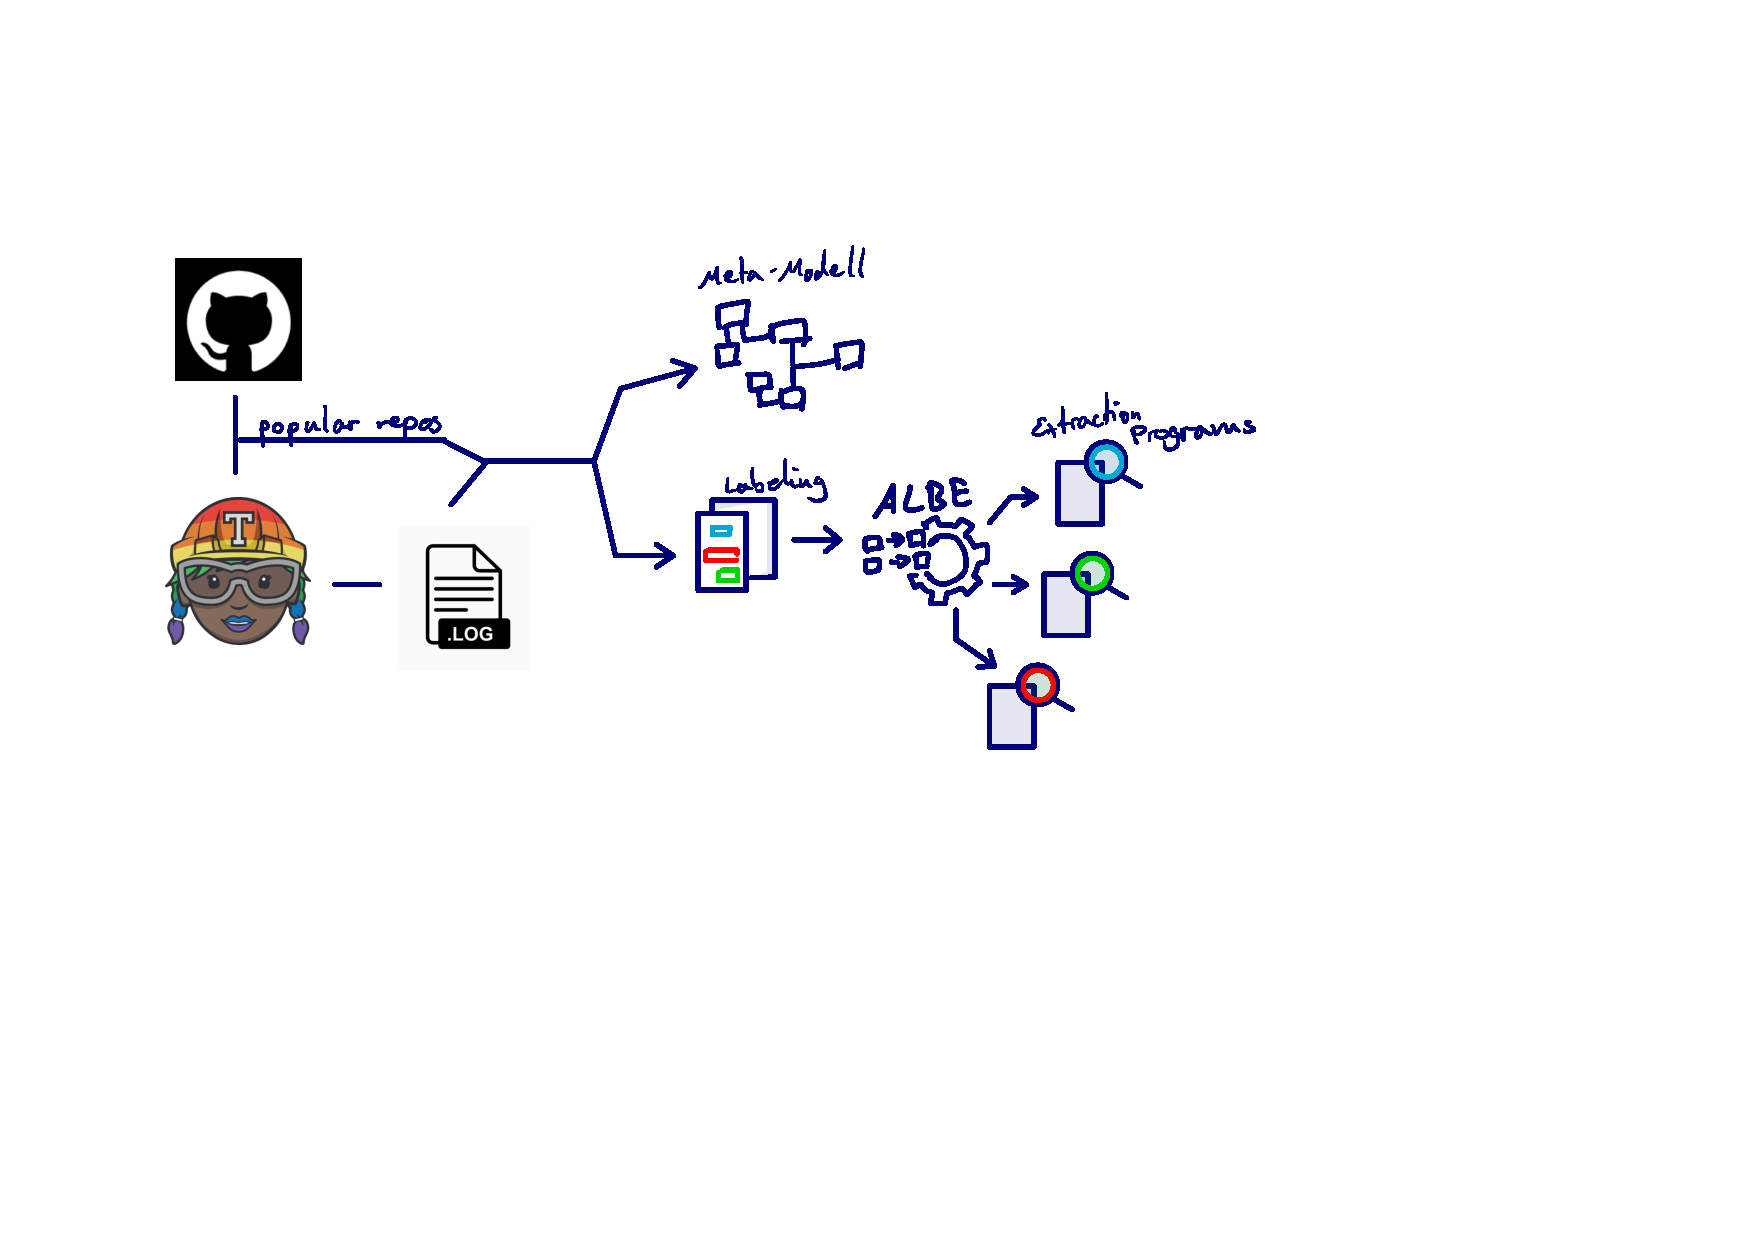
\includegraphics[width=0.5\textwidth, trim={0.5cm 5cm 3cm 2cm}, clip]{img/flow-of-research.pdf}
	\caption{Flow of Research}
\end{figure}

\subsection{Data collection}

\draft{
In order to build a tool which facilitates information extraction from build logs we first had \todo{which time form here? past or present?} to get an impression on what kinds of build logs occur in projects, what possibly extractable information they contain and how structured or unstructured they are.
}

\subsubsection{Design} ...
\bp{
realistic image (for open source software) we sample from popular GitHub repositories that also use Travis CI.

\draft{Obtaining the newest logs from them would entail sampling mostly logs of succeeding builds as the distribution of build states on a Travis CI repository is highly skewed towards successful builds~\cite{beller2017oops}. Therefore we stratify our collection of logs and select an equal amount of logs from each type of Travis CI build status.}
}

\subsubsection{Execution} ...
\bp{
built tool X \todo{data collection tool name, LogCollector?}

queryed ghtorrent dataset from the first of April 2018 through google BigQuery

poked Travis CI for active status of project and collected sampled builds through Travis ruby library

downloaded logs through Travis Rest API \todo{look up version}
}


\subsection{Meta-Model}
\bp{through manual examination of y of the build logs we collected designed a meta-model  of the contained/extractable/useful/interesting information}

\todo{figure with meta-model}
\begin{figure}
	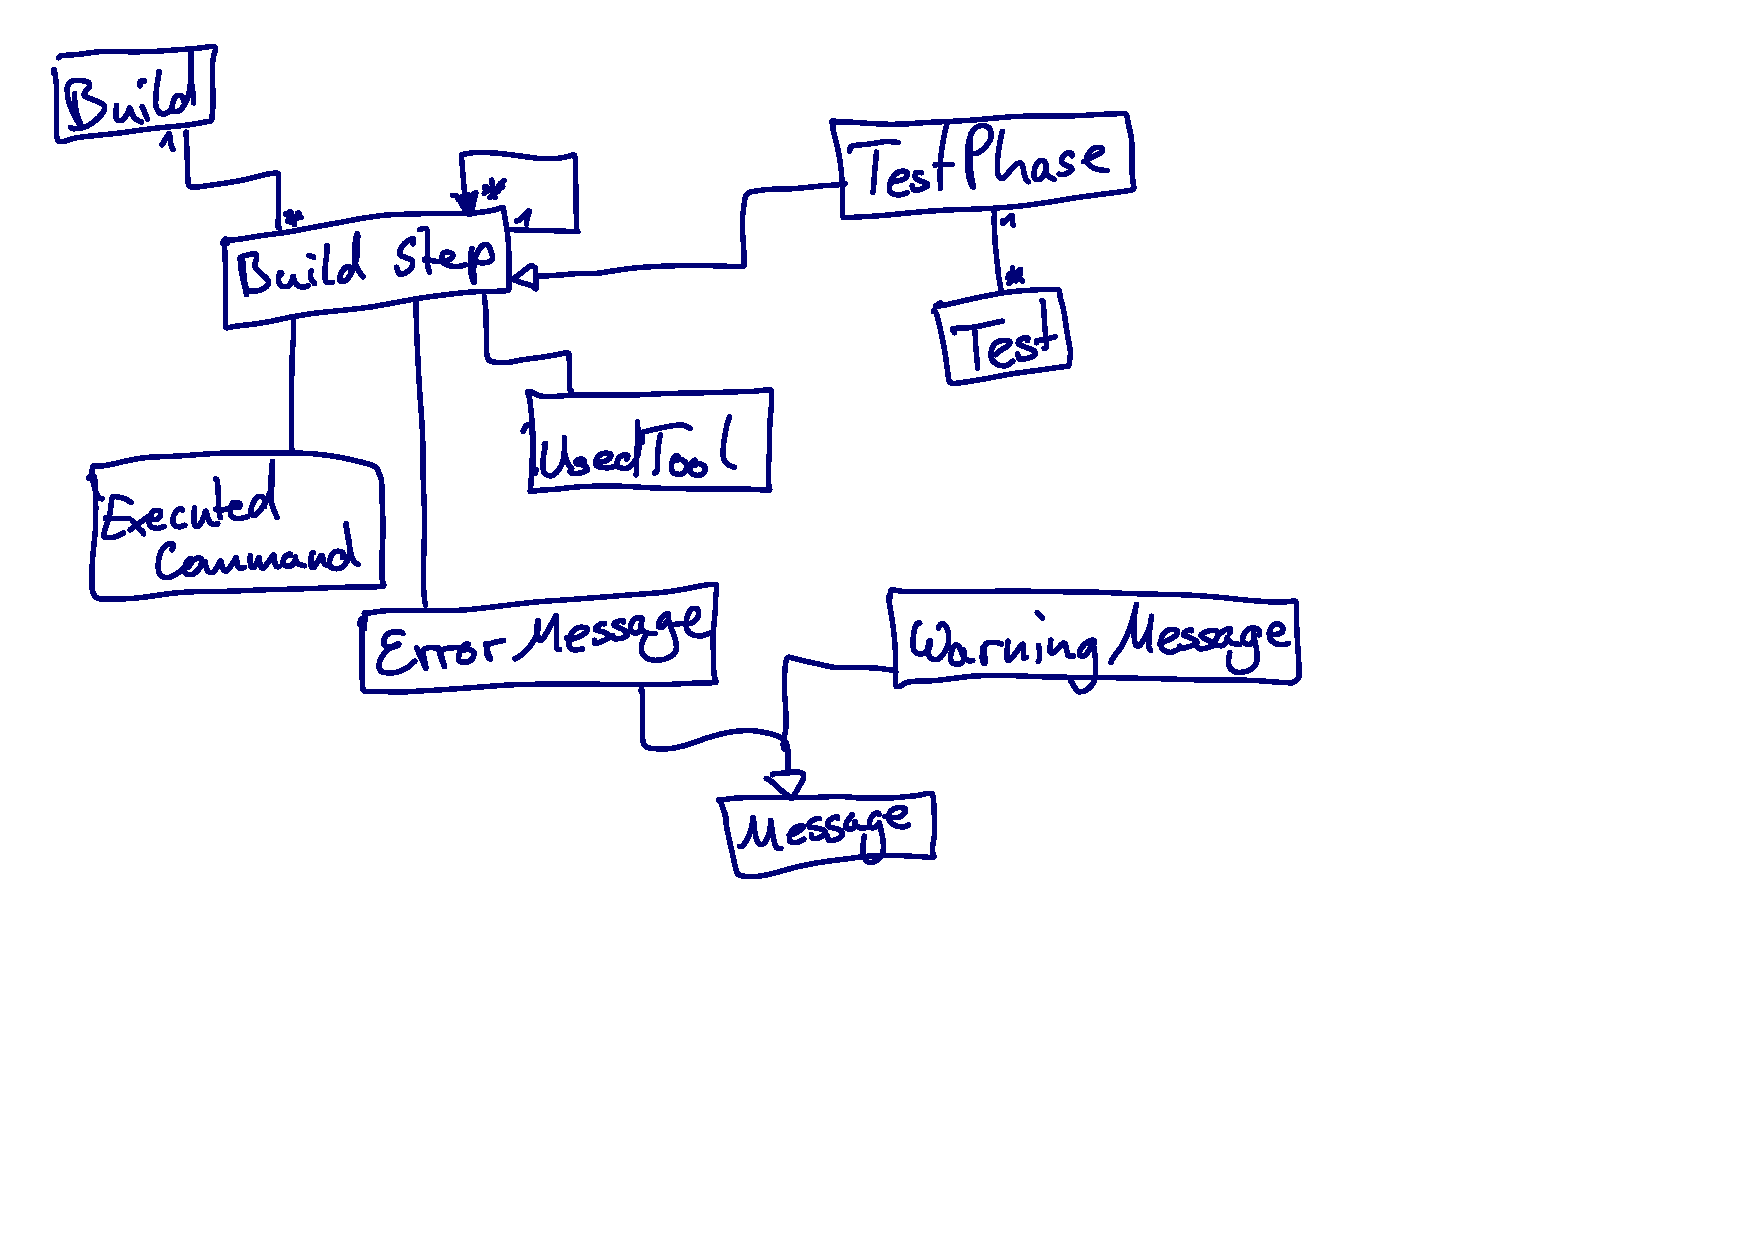
\includegraphics[width=0.5\textwidth, trim={0.5cm 4cm 3cm 0.5cm}, clip]{img/meta-model.pdf}
	\caption{Meta-Model}
\end{figure}

\plan{explain (shortly? partly?) meta model classes}

\subsection{Our Tool: ALBE \textemdash \ Analyzing Logs By Example}

\plan{
techstacky: C\#, dot net core, Microsoft PROSE library specifically their TextExtraction DSL

samples \& learning: labeled data is in xml files, parsed (and shuffled) for examples, program learned for specific instruction

interaction: user can analyze given file with program defined by specific exampleset, if there: describe how to use iteratively growing / shuffling learning process
}

\subsubsection{Capabilities} ...

\plan{
Example extractions: travis worker, android failure, what we do evaluations on
}

\subsubsection{Limitations} ...

\plan{
Travis worker both kinds at once, explain PROSE limitations on arbitrary OR regexes

for all limitations: why? and how would we solve that?
}

\subsection{Evaluation}
\bp{
To evaluate our tool we did xyz, we wanted to measure: accuracy of extractions, impression on effort of creating such extraction, compare both to existing methods
}


\subsubsection{Extraction Accuracy}
...

\bp{we labelled x logs from project y using language z / build tool b. (do for one, maybe extend with further one) 

evaluated accuracy \todo{<define accuracy for us>} with growing number of 
\begin{itemize}
	\item random selected
	\item chronologically sampled
	\item hand selected 
\end{itemize}
samples.
}

\subsubsection{Compare to Traditional Methods}
\paragraph{TravisTorrent} ...
\bp{Beller et al. \mention{cite correct travistorrent paper} reported on manually constructing a parser with regular expressions for ruby \& Java and common build tools / output formats there, they can extract \todo{<explain there extractions, with example necessary?}
	
android-failure example: decided not to implement as to complicated \todo{<- that kind of already belongs into results, how do we describe the \emph{method} of this comparison accurately??}
}

\paragraph{Manual Regex Construction} ...
\plan{
for something where I did not look at the synthesized program

alternative: small study with other developers on manual vs. pbe extraction
}

\paragraph{IR paragraph stuff} ...
\plan{
maybe simple setup with lines implementing vector comparison on keywords ourselves -> how can we reuse the labeling for the c\# tool?
}

\paragraph{Keyword search} ...
\plan{
either: we give a list of keywords generally associated with the thing we want to extract (e.g. failure/error/..) -> write nicely how we brainstormed that

or: small study of what developers would search for (maybe literature already did that?)

or: relate to samples? search for already seen words from last failure
}

\section{Results}
\secfunc{hard numbers! answers to research questions, narrow}

\plan{graphs!, achieved accuracy, samples needed for same accuracy as related tools (travistorrent), aging of learned programs with newer data}

\section{Analysis / Discussion}
\secfunc{interpretation, implication of answers and why does it matter, comparison to previous findings, narrow $\rightarrow$ wide}

\plan{our tool works well for defined cases, limitations of tool/prose/regex usage in general, every x weeks extraction has to be rewritten to keep accuracy, well improved if only y new examples have to be added}

\section{Conclusion and Future Work}
\secfunc{summarize, results again, future research}

\plan{repeat everything and results}

\plan{future}

\bp{make avaliable to other researchers

integrate into travis

\plan{as always} extend evaluation and data collection

use dataset to evaluate against existing approaches

}

%%
%% The acknowledgments section is defined using the "acks" environment
%% (and NOT an unnumbered section). This ensures the proper
%% identification of the section in the article metadata, and the
%% consistent spelling of the heading.
\begin{acks}
To Robert, for the bagels and explaining CMYK and color spaces.
\end{acks}

%%
%% The next two lines define the bibliography style to be used, and
%% the bibliography file.
\bibliographystyle{ACM-Reference-Format}
\bibliography{paper}

%%
%% If your work has an appendix, this is the place to put it.
\appendix

\section{Research Methods}

\subsection{Part One}


\end{document}
\endinput
%%
%% End of file `sample-sigconf.tex'.
